\chapter{Desenvolvimento}
\label{metodo}

Este capítulo ....
Apresentar uma classificação da pesquisa.

\section{Biblioteca de manipulação de grafos}
Como primeira etapa foi desenvolvida uma biblioteca de manipulação de grafos que será utilizada futuramente nas próximas etapas.

A biblioteca de manipulação é composta por um conjunto de funções e métodos que manipulam tanto um grafo representado em matriz, quanto um grafo representado por lista de adjacência.

Para um bom design de solução, que fosse reutilizável e compreensível, foi utilizada a linguagem Java como principal ferramenta. A arquitetura desenvolvida para a biblioteca, nos dá a liberdade para escolher qual estrutura de dados manipular e utilizar de módulos de geração, leitura e salvamento de grafos de maneira separada.

A Biblioteca como um todo é composta por duas classes principais que guardam as estruturas de dados de Grafos em matriz e em lista de adjacência. A primeira classe é chamada de GraphMatrix, responsável por manipular e armazenar um grafo não-direcionado em uma matriz de N linhas por N colunas tal que N é o número de vértices do grafo. A segunda classe se chama apenas Graph e ela herda todas as características de GraphMatrix. Graph, é responsável por manipular e armazenar tanto grafo em matriz, quanto o grafo em lista de adjacência.

Além das classes principais, existem outros dois módulos que auxiliam nos testes e desenvolvimento. Sendo o primeiro deles chamado de GraphIO, utilizado na leitura e salvamento de grafos em arquivos no formato Pajek NET, e o segundo módulo, chamado de GraphGenerator, responsável por gerar grafos com base na quantidade de vértices, número mínimo de grau por vértice e número máximo de grau por vértice.

Para garantir que todos os algoritmos estão funcionando corretamente e retornando resultados esperados, foram desenvolvidas baterias de teste para cada uma das funções do sistema. Assim, é possível ter certeza e confiar que tanto o processamento que ocorre nas matrizes, quanto os que ocorrem nas listas entregam os mesmos resultados de adição e remoção de arestas, ponderação de vértices e arestas, e para todas as outras funções. Os testes foram escritos utilizando a biblioteca Junit do próprio Java.

A Organização de todo o sistema pode ser representada pelo seguinte diagrama de classe:

\begin{figure}[ht]
	\centering	
	\caption[\hspace{0.1cm}Diagrama Classe]{Diagrama de Classe}
	\vspace{-0.4cm}
	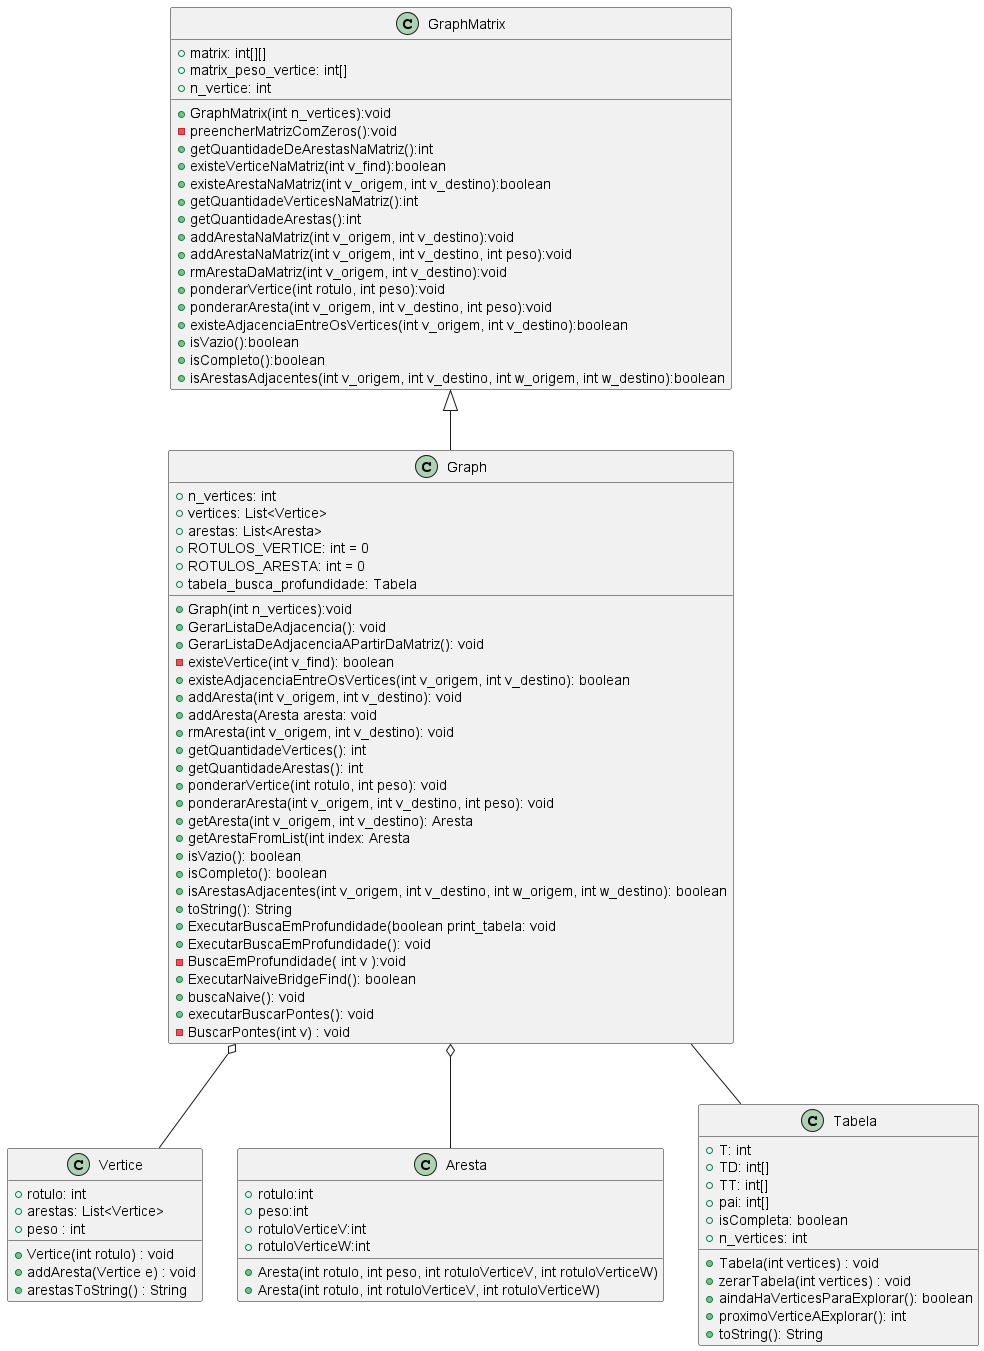
\includegraphics[width=0.6\textwidth]{DiagramaDeClasse/DiagramaDeClasse.png}
	% Caption centralizada
% 	\captionsetup{justification=centering}
	% Caption e fonte 
	 \vspace{-0.2cm}
	\\\textbf{\footnotesize Fonte: \cite{imagemSoftware} }
	\label{fig:imagemSoftware}
\end{figure}

\subsection{Atividade 1: xxxx}
Descrição

\subsection{Atividade 2: xxxx}
Descrição

\subsection{Atividade n: xxxx}
Descrição

\section{Cronograma}
%\addcontentsline{toc}{chapter}{Cronograma}

Esta seção apresenta ... (Tabela \ref{tab-crono}).

\begin{table}[h]
\centering
\caption{Cronograma}
\label{tab-crono}
\begin{tabular}{|l|l|l|l|l|}
\hline
                 &
                 \textbf{\begin{tabular}[c]{@{}l@{}}Meses\\ 1-3\end{tabular}} & \textbf{\begin{tabular}[c]{@{}l@{}}Meses\\ 4-6\end{tabular}} &  
                 \textbf{\begin{tabular}[c]{@{}l@{}}Meses\\ 7-9\end{tabular}} & 
                 \textbf{\begin{tabular}[c]{@{}l@{}}Meses\\ 10-11\end{tabular}}  \\ \hline
Pesquisa asdads & X                                                          & X                                                           &  &  \\ \hline
Coleta de dados     &                                                            & X                                                         & X &  \\ \hline
sdfsdf           &                                                         X   &                                                            & X & X \\ \hline
nova linha           &                                                         X   &                                                            & X & X \\ \hline
\end{tabular}
\end{table}